\documentclass{rapportCS}
\usepackage{lipsum}
\usepackage{amsmath}
\usepackage{amsfonts}
\usepackage{amssymb}
\usepackage{enumitem}
\setlist[itemize]{topsep=0pt, itemsep=0pt}

\title{End-of-Studies Internship Report Martini}

\begin{document}
 
%----------- Informations du rapport ---------

\logoentreprise{logos/logoICM.png} %Logo de l'entreprise

\titre{Developping simulation and statistical evaluation tools for a non-linear mixed-effect models}

\mention{CentraleSupélec - Mention Sciences des données et de l'information \& Filière Métiers de la Recherche}
\master{Master MVA} % Nom du master
 

\eleve{Jean-Vincent Martini}  
 
\dates{April 2026 - September 2026}   
 
% Informations tuteurs écoles
\tuteurecole{
    SDI: \textsc{Arthur Tenenhaus} \\
    arthur.tenenhaus@l2s.centralesupelec.fr \\
    FMR: \textsc{Vincent Mousseau} \\ 
    vincent.mousseau@centralesupelec.fr
} 

\tuteurentreprise{
    \textsc{Sophie Tezenas du Montcel} \\
    sophie.tezenas@aphp.fr 
}

%----------- Initialisation -------------------
        
\fairemarges %Afficher les marges
\fairepagedegarde %Créer la page de garde
\setcounter{figure}{0}

%----------- Abstract -------------------
\begin{abstract}
        TODO
\end{abstract}
\newpage

%------------ Table des matières ----------------

\tableofcontents
\newpage   

%------------ Introduction ----------------

\section{Introduction} 
TODO  

\newpage 

%------------ Sections ----------------

\section{Context and Related Work}

Neurodegenerative diseases are characterized by a slow and complex evolution, involving numerous heterogeneous clinical and biological markers (biomarkers, imaging, clinical scores) that evolve jointly over time. Modeling and predicting this progression from multivariate longitudinal data is a central challenge for clinical research and precision medicine.

In this context, Leaspy (LEArning Spatiotemporal Patterns in Python), an open-source Python library, was developed by the ARAMIS team at the Paris Brain Institute (ICM) in collaboration with INRIA, INSERM, CNRS and Sorbonne University to analyze the joint evolution of numerous markers simultaneously. The repository is available at \url{https://github.com/aramis-lab/leaspy} and the documentation at \url{https://leaspy.readthedocs.io/en/stable/index.html}. 

The package is designed for the statistical analysis of longitudinal medical data consisting of repeated observations of patients at different time points. Its principal use cases include: reconstructing the long-term spatiotemporal trajectory of disease evolution from short-term cohort data; positioning individual patients relative to a group-average disease timeline; quantifying the impact of cofactors (sex, genetic mutations, environmental factors) on progression; imputing missing values; predicting future observations; and simulating virtual patient cohorts.

\subsection{Mathematical Background}

\subsubsection{Nonlinear Mixed-Effects Models}

Leaspy is based on the non-linear mixed-effects models framework, which decomposes variability in longitudinal observations into two complementary components~\cite{schiratti2017bayesian}:

\begin{itemize}
  \item \textbf{Fixed effects} (population-level): systematic trends shared across all individuals, such as the average disease trajectory, typical progression speed, and population reference time.
  \item \textbf{Random effects} (individual-level): subject-specific deviations capturing heterogeneity in onset time, progression speed, and the relative ordering of biomarker changes.
\end{itemize}

Formally, let $y$ denote the observed data, $z = (z_{\mathrm{fe}}, z_{\mathrm{re}})$ the latent fixed and random effects, $\theta$ the model parameters, and $\Pi$ the known hyperparameters. Parameter estimation is performed by maximizing the marginal likelihood
\begin{equation}
  p(y \mid \theta, \Pi) = \int_{z} p(y, z \mid \theta, \Pi)\, dz,
\end{equation}
which decomposes in log-space as
\begin{equation}
  \log p(y, z \mid \theta, \Pi)
    = \underbrace{\log p(y \mid z, \theta, \Pi)}_{\text{data attachment}}
    + \underbrace{\log p(z_{\mathrm{re}} \mid z_{\mathrm{fe}}, \theta, \Pi)
                + \log p(z_{\mathrm{fe}} \mid \theta, \Pi)}_{\text{prior attachment}}.
\end{equation}

Because this integral is intractable in closed form, Leaspy employs the MCMC-SAEM algorithm (Markov Chain Monte Carlo Stochastic Approximation Expectation-Maximization) \cite{kuhn2005maximum}. This algorithm alternates between (i) a stochastic approximation step that uses Gibbs sampling to draw latent variables conditional on current parameter estimates, and (ii) a maximization step that re-estimates fixed effects and variance components from the updated sufficient statistics.

\subsubsection{Riemannian Geometry of Disease Progression}

A key innovation of Leaspy is the interpretation of disease progression within a Riemannian geometric framework~\cite{schiratti2017bayesian}. The core idea is to represent the multivariate progression of clinical markers as a geodesic on a product Riemannian manifold, where the shape of the curve is entirely determined by the choice of the metric $G(p)$. 

For clinical scores exhibiting floor or ceiling effects, common in neurodegenerative disease assessment, the manifold $(0,1)$ equipped with the metric $G(p) = 1/[p^2(1-p)^2]$ yields logistic (sigmoidal) trajectories. This metric encapsulates the bounded nature of the scores in a geometrically principled way. More generally, the Euclidean metric on $\mathbb{R}^n$ yields linear trajectories, allowing the framework to accommodate diverse data types.

The average population trajectory $\gamma_0$ is a geodesic parameterized by its initial conditions at reference time $t_0$: initial position $p_0 = \gamma_0(t_0)$ and initial speed $v_0 = \dot{\gamma}_0(t_0)$. Individual trajectories $\gamma_i(t)$ are derived from this average through three types of random effects:

\begin{itemize}
  \item \textbf{Time shift} $\tau_i$: earlier or later disease onset relative to the population average.
  \item \textbf{Log-acceleration factor} $\xi_i$: faster or slower progression speed.
  \item \textbf{Space shifts} $w_{i,k}$: modifications to the relative ordering and timing of individual biomarker progressions, encoded as tangent-space perturbations.
\end{itemize}

These three effects are combined through a latent disease age reparametrization:
$\psi_i(t) = v_0\, e^{\xi_i}(t - \tau_i) + t_0$, which transforms the calendar age $t$ of patient $i$ into a disease-stage age. This reparametrization provides a biologically interpretable decomposition: $\tau_i$ captures onset heterogeneity, $e^{\xi_i}$ captures progression rate heterogeneity, and the space shifts $w_{i,k} = (\mathbf{A}\mathbf{s}_i)_k$, obtained via the mixing matrix $\mathbf{A}$ acting on independent sources $\mathbf{s}_i$, capture differences in the sequential ordering of biomarker changes across patients.

\subsection{Main Models}

\paragraph{Logistic Model.} The logistic model is the core model of Leaspy, designed for multivariate longitudinal data whose components exhibit sigmoidal (bounded, monotone) progressions, typical of cognitive scores or normalized biomarkers.

\paragraph{Joint Model.} The joint model \cite{ortholand2025joint} extends the logistic model to simultaneously analyze longitudinal measurements and time-to-event data (survival, clinical events, competing risks). Rather than treating these processes separately, which can lead to biases from informative dropout, the joint model links them through the shared latent disease age $\psi_i(t)$, avoiding the need to define an explicit disease reference time.

\paragraph{Mixture Model.} Standard mixed-effects models assume a single population trajectory with random individual deviations. The mixture model \cite{kaisaridi2025mixture} relaxes this assumption by modeling the population as a combination of $n_c$ latent subgroups, each with its own distribution of individual parameters. This formulation enables simultaneous disease progression modeling and probabilistic patient subtyping.

\subsection{Main Algorithms}

Leaspy provides four main algorithmic operations:
\vspace*{-0.4cm}
\paragraph{\texttt{fit}:} Estimates population parameters (fixed effects and variance components) from a cohort of longitudinal observations using MCMC-SAEM. The user specifies the model type, number of outcomes, number of latent sources, and observational noise model. The result is a fitted model characterizing the average disease trajectory and its population-level variability.
\vspace*{-0.4cm}
\paragraph{\texttt{personalize}:} Given a fitted model, estimates individual random effects $(\tau_i, \xi_i, \mathbf{s}_i)$ for each subject from their available observations. Two approaches are available: a frequentist mode using \texttt{scipy.optimize.minimize} to maximize the individual likelihood, and a Bayesian mode using a Gibbs sampler to extract the mean or mode of the posterior distribution. The output is a set of individual parameters that characterize each patient's position on the disease timeline.
\vspace*{-0.4cm}
\paragraph{\texttt{estimate}:} Evaluates the modeled trajectory $\gamma_{i,k}(t)$ for a specific patient at arbitrary time points, using the previously estimated individual parameters. This enables reconstruction of the full disease trajectory, imputation of missing values, and forecasting of future clinical scores.
\vspace*{-0.4cm}
\paragraph{\texttt{simulate}:} Generates synthetic patient cohorts by (i) sampling individual parameters from the learned population distributions, (ii) generating visit times according to user-specified schedules (random, regular, or custom), and (iii) evaluating model trajectories with added observational noise. This functionality is only available for the logistic model for now, but a part of this work consists in extending it to the joint model.

\subsection{Applications and Related Work}

Leaspy has been applied to  neurodegenerative diseases, demonstrating its generalizability and clinical relevance.
\vspace*{-0.2cm}
\paragraph{Parkinson's disease.}
Leaspy comes with a built-in Parkinson's disease dataset, enabling out-of-the-box demonstration and benchmarking. Figure~\ref{fig:parkinson} illustrates the typical results obtained with the software.

\begin{figure}[htbp]
  \centering
  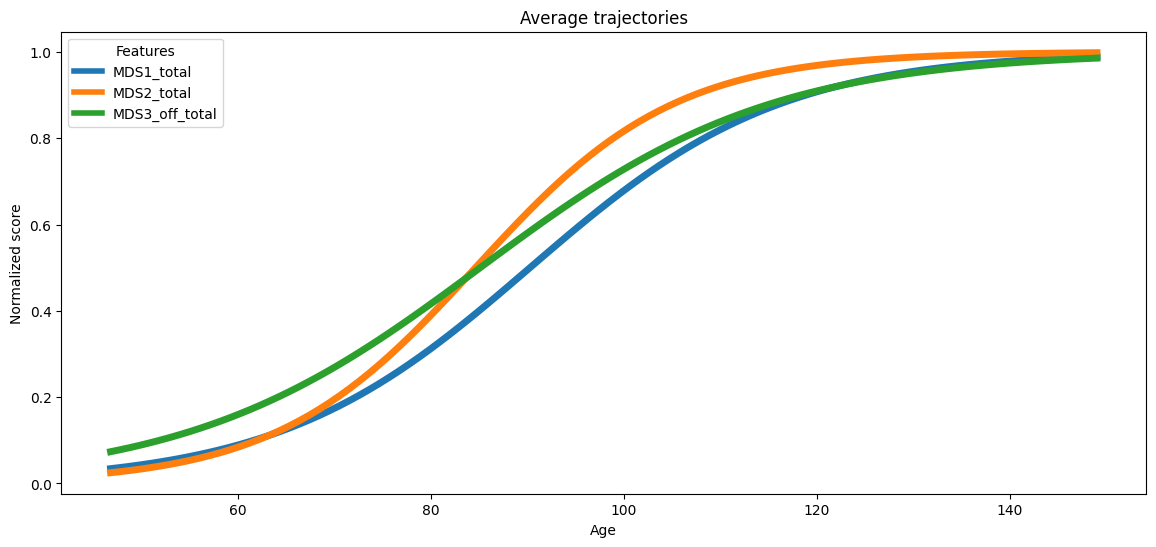
\includegraphics[width=0.41\textwidth]{figures/avg_example.png}
  \hfill
  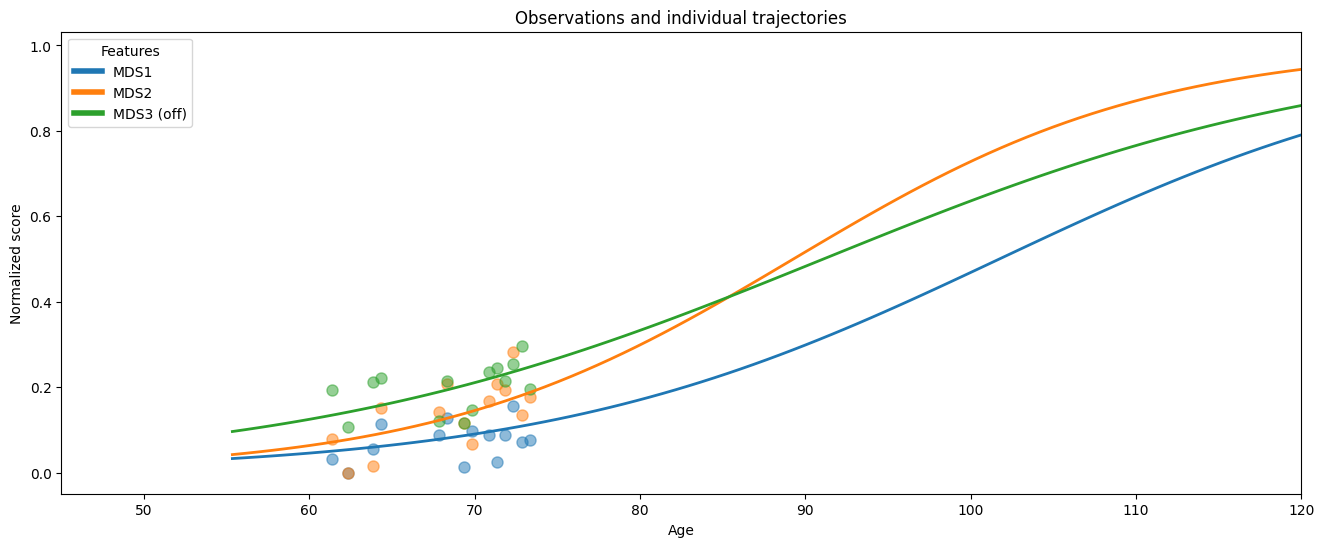
\includegraphics[width=0.48\textwidth]{figures/obs_example.png}
  \caption{Disease progression modeling with Leaspy on the built-in Parkinson's dataset. \textbf{Left:} Average population trajectory of clinical scores over the estimated disease timeline. \textbf{Right:} Personalized trajectory (solid line) and observed visits (dots) for one patient.}
  \label{fig:parkinson}
\end{figure}
\vspace*{-0.2cm}
\paragraph{Alzheimer's disease (AD).} The AD Course Map~\cite{koval2021ad} uses Leaspy to create a spatiotemporal atlas of AD progression by jointly modeling neuropsychological and imaging data. It outperformed 56 competing methods in the TADPOLE open challenge and, when tested globally on over 4,600 patients, demonstrated the ability to enrich clinical trials with predicted progressors, reducing required sample sizes by up to 50\%~\cite{maheux2023forecasting}.
\vspace*{-0.2cm}
\paragraph{Huntington's disease.} Koval et al.\ applied the disease course mapping framework to identify the optimal intervention window for Huntington's disease clinical trials, demonstrating that the model could ``spot the time to treat'' by positioning patients on the disease timeline prior to symptom onset~\cite{koval2022forecasting}.
\vspace*{-0.2cm}
\paragraph{CADASIL.}
Kaisaridi et al.\ applied Leaspy to 395 patients from the French CADASIL referral center, modeling the joint progression of 14 clinical scores. Using a mixture model, they identified two clinically meaningful subgroups, an early-onset, rapidly progressing group and a late-onset, slowly progressing group, providing new insights into disease heterogeneity for this rare small vessel disease~\cite{kaisaridi2025mixture}.
\vspace*{-0.2cm}
\paragraph{Amyotrophic lateral sclerosis (ALS).}
The joint model was validated on data from patients with ALS from the PRO-ACT dataset. The spatiotemporal model links longitudinal clinical decline to time-to-ventilation and survival events, outperforming standard shared-random-effect joint models in accuracy and discriminative ability while using fewer parameters~\cite{ortholand2025joint}. 

\newpage

%------------ Bibliography ----------------

\bibliographystyle{plain}
\bibliography{bibliography}

\end{document}
